% Do not forget to include Introduction
%---------------------------------------------------------------
% \chapter{Introduction}
% uncomment the following line to create an unnumbered chapter
\chapter*{Úvod}\addcontentsline{toc}{chapter}{Úvod}\markboth{Úvod}{Úvod}
%---------------------------------------------------------------
\setcounter{page}{1}

Technologický pokrok je nezadržitelný. Nové poznatky umožňují rychlý vývoj sofistikovaného technického vybavení výpočetních číslicových elektronických strojů --- sálových, domácích i~mobilních univerzálních i~specializovaných počítačů, vestavěných řídicích systémů a~dalších zařízení.

Spolu s~technologickým pokrokem přichází mnoho nových informací. Důležitou součástí procesu učení je informace nejen získat, ale i~zpracovat a~porozumět jim, jelikož \enquote{formální osvojování jakýchkoliv faktů bez porozumění se zákonitě promítá do nízké rychlosti i~ekonomičnosti učení a~malé trvalosti paměťové stopy, včetně praktické nevyužitelnosti.}~\cite{Zacharova2012:psychologie}

V~mnoha oblastech však obecné principy zůstávají podobné, ne-li stejné. Přirozeně se tudíž k demonstraci principů nabízí využít jednoduššího systému. Takový systém můžeme získat vytvořením modelu aktuálních složitých systémů, což se prakticky využívá například v~systémech reálného času~\cite{Kubatova2019:src-modely}. Jinou variantou řešení se zabývá tento text; využitím historického systému.

Historické systémy, podobně jako ty moderní, vychází z teoretických matematických konceptů (například programovatelný počítač vycházející z Turingova stroje~\cite{Teuscher2003:turing}). Zároveň jsou poměrně jednoduché, jelikož vznikaly s~technologickými omezeními. Není tedy potřeba vytvářet abstraktní model, ale demonstrovat principy na existujícím systému, což může zvýšit atraktivitu i~užitečnost předávaných informací.

Jedním ze způsobů, jak takový systém přiblížit jakémukoliv zájemci o problematiku, je přenést jej do softwaru, který bude možné spustit na běžně dostupných počítačích. Jednou z možností je takzvaná emulace; výsledný software je nazýván emulátor.

Cílem bakalářské práce je vytvořit emulátor historické herní konzole \emph{Nintendo Entertainment System}. Jelikož je kladem důraz na využití ve výuce, je nutnou součástí návrhu vývoj univerzální platformy, která takový systém zvládne nejen emulovat, ale zároveň zobrazovat informace o~vnitřním stavu systému, jakožto i~umožnit jednoduché modifikace a~přidávání funkcionalit.

Implementační část, hotová emulační platforma, je pouze dílčí výsledek práce. Samotný vývoj emulovaných komponent přináší mnoho zajímavých problémů k~řešení, proto je namístě tento proces důkladně dokumentovat a~vytvořit tak příklad pro uživatele, kteří by chtěli příkladnou implementaci rozšířit, případně na platformě vyvinout emulátor jiného systému. Dílčím cílem práce je tedy seznámit čtenáře s~vývojem a~motivovat jej  ještě důkladněji zkoumat prezentované principy.

Práce je členěna na několik hlavních částí:
\begin{description}
	\item[Představení problematiky] V~této kapitole je představena problematika emulace v~teoretické rovině --- definují se potřebné pojmy. Kapitola popisuje jednak emulaci obecně, jednak konkrétní emulované komponenty.
	\item[Analýza] Analytická, stěžejní kapitola práce, seznámí čtenáře s~uvažovanými variantami řešení. Dochází k~analýze existujících implementací a~k~výběru vhodných technologií a~metodik vzhledem k~emulovaným komponentám.
	\item[Implementace] Implementační kapitola je popisem procesu tvorby emulační platformy a emulovaných komponent.
	\item[Testování] Předposlední kapitola je zaměřena na testování projektu. Popisuje nejen průběžné testování aplikace, ale i~porovnání věrnosti s~reálným systémem. metodou spouštění necertifikovaného kódu na originálním hardwaru.
	\item[Navazující práce] Poslední kapitola je věnována shrnutí zbývajících funkcionalit, které budou implementovány v~dalších verzích emulační platformy. Slouží také jako pobídka dalším uživatelům-vývojářům, kteří by měli zájem projekt rozšířit v~rámci sebevzdělávání.
\end{description}

\begin{note*}[Terminologie]
	Jelikož je bakalářská práce zaměřena na vzdělávací využití, kombinuje odbornost s~populárně-naučným formátem. Počítá se s~faktem, že čtenář se v~oboru informačních technologií již pohybuje, proto se používají anglické termíny tam, kde je to běžné. Nemělo by tedy například čtenáře zaskočit, že se občas jako \emph{programové vybavení} počítače označuje výrazem \emph{software} a~\emph{technické vybavení} počítače jako \emph{hardware}.
\end{note*}

\begin{note*}[Značení]
	V~textu se často používají čísla v šestnáctkové soustavě, jelikož úsporně reprezentují například paměťové adresy. Takové číslice se značí předponou amerického dolaru: \$. Desítková čísla jsou uvedena bez předpony.
	
	Dále se používají různé zkratky; jsou uvedeny v~seznamu zkratek. Neobvyklé zkratky se před jejich použitím v~textu vysvětlují.
\end{note*}

%---------------------------------------------------------------
\chapter{Představení problematiky}
\label{chap:predstaveni-problematiky}
%---------------------------------------------------------------

\epigraph{
	\enquote{We can only see a short distance ahead, but we can see plenty there that needs to be done.}
}{\textit{Computing Machinery and Intelligence}\\ \textsc{Alan Turing}}

\section{Emulace}
V úvodu byl použit pojem emulátor. Pro začátek je tedy vhodné tento pojem oficiálně zavést.

\begin{definition}[Emulátor]
	Emulátor je druh softwaru, který umožňuje běh počítačových programů na jiné platformě, než pro kterou byly původně vytvořeny~\cite{Wikipedia:emulator}.
\end{definition}

\begin{note}[Emulovatelnost]
	Dává smysl se zabývat vytvářením emulátoru, jelikož lze pro každý software vytvořit příslušný emulátor. Lze se odkázat na Churchovu-Turingovu tezi, ze které vyplývá, že ke každému algoritmu existuje ekvivalentní Turingův stroj.
\end{note}

Dle jiné definice pod pojem emulátor spadá i~hardwarové řešení emulátoru. Tímto se však práce nezabývá, proto bude dále brána v~potaz jen již uvedená softwarová emulace.

Emulace se od podobného pojmu, \emph{simulace}, liší především tím, že se na emulátoru spouští originální programové vybavení emulovaného systému. Nedochází tedy k~napodobení funkce, ale celého hardwaru tak, aby byl schopný věrně interpretovat původní program. V~případě této práce se jedná o~interpretaci instrukcí původně obsaženého v paměti ROM.

\begin{example}
V~kontextu herních konzolí lze uvést rozdíl na následujícím příkladu. Simulace by napodobila vzhled a~chování každé jednotlivé hry. Například simulátor příruční herní konzole s~vestavěnou hrou \emph{Tetris} by byla nová implementace hry bez ohledu na hardware, který byl v~konzoli použit. Emulátor by naopak nebral žádný ohled na jakýkoliv software, ale snažil by se věrně napodobit hardwarové vybavení konzole tak, aby bylo možné kopii softwaru (hru) spustit beze změn. Takto je možné provozovat na emulátoru jakékoliv programové vybavení kompatibilní s~daným hardwarem \cite{FulberGarcia2022:simulation-emulation}
\end{example}

\subsection{Způsoby emulace}
Emulaci je možné dělit dle úrovně, na které emulátor pracuje, což je úzce spjato s~teorií počítačových architektur. Na úvod je vhodné se zamyslet nad programováním fyzického počítačového systému, což poskytne přehled o~dostupných zdrojích informací pro vývoj emulátoru. Tato podkapitola tedy odpoví na dvě otázky:
\begin{enumerate}
	\item V~jaké formě bude spouštěný software?
	\item Na jaké úrovni se tento software zpracuje?
\end{enumerate}

Běžné počítačové systémy odpovídají teoretickému modelu programovatelného počítače.

\begin{definition}[Programovatelný počítač]
	Programovatelný počítač je takový počítač, který čte instrukce z~elektronické paměti, kde jsou uloženy.~\cite{Wikipedia:programovatelny-pocitac}
\end{definition}

Komponentou počítače, která je zodpovědná za řízení, je většinou \emph{procesor}. Proto má smysl se nejdříve zamýšlet nad úrovní abstrakce procesoru, jelikož je to právě ta komponenta, která bude zpracovávat programy a~řídit komponenty ostatní.

Instrukce bývají v paměti číslicových počítačů reprezentovány jako strojový kód, který většinou vzniká překladem z~jazyka vyšší abstrakce (například JSA)~\cite{Kubatova2018:SAP}, což ilustruje diagram~\ref{fig:abstrakce-sw}. Jelikož je strojový kód nativní způsob zpracování instrukcí a~zároveň se v~této formě běžně distribuuje software, emulátor by měl pracovat právě s~touto reprezentací. Tím se získala odpověď na první otázku.

\begin{figure}[ht!]
	\centering
	\caption{~Úrovně abstrakce softwaru}\label{fig:abstrakce-sw}
	\begin{tikzpicture}[node distance=2cm] 
		\tikzstyle{uroven} = [rectangle, rounded corners, minimum width=5cm, minimum height=1cm,text centered, draw=black]
		\tikzstyle{arrow} = [thick,->,>=stealth]
		
		\node (vyssijazyk) [uroven] {Vyšší programovací jazyk};
		\node (jsa) [uroven, below of=vyssijazyk] {Jazyk symbolických instrukcí};
		\node (strojkod) [uroven, below of=jsa, fill=headbackgroundgray] {Strojový kód};
		\node (signaly) [uroven, below of=strojkod] {Řídící signály};
		
		\draw [arrow] (vyssijazyk) -- (jsa);
		\draw [arrow] (jsa) -- (strojkod);
		\draw [arrow] (strojkod) -- (signaly);
	\end{tikzpicture}
\end{figure}

Druhá otázka se již zabývá přiřazení smyslu jednotlivým instrukcím. Množina podporovaných instrukcí včetně dalších potřebných informací (především o způsobu reprezentace a ukládání dat) je součástí architektury procesoru (ISA)~\cite{Kubatova2018:SAP}.

Z výše uvedeného vyplývá, že pro zpracování instrukcí tak, jako to dělal původní hardware, stačí jen přesně napodobit chování jednotlivých instrukcí dle popisu architektury, bez dalšího zamýšlení se, jak je procesor konkrétně implementován. To představuje nejvyšší úroveň abstrakce. 

Některé programy se však občas spoléhají na nedokumentované chování procesorů, kde je již nutné pracovat na nižší úrovni. Dle prof. Kubátové se jedná o úroveň předávání dat mezi registry, na které pracuje i~emulátor bakalářské práce.

Existují ještě dvě nižší úrovně, úroveň logických hradel a~úroveň tranzistorů~\cite{Kubatova2018:SAP}. Tyto dvě úrovně již však vyžadují znalost konkrétní hardwarové implementace, která bývá obchodním tajemstvím. Výhodou je, že ve své podstatě nevyžaduje vůbec znalost o~funkci procesoru jako takovém a~zároveň nejvěrněji implementuje jeho funkčnost. Velkými nevýhodami jsou obtížnost, častá absence potřebných informací a~při implementaci v softwaru i~velká náročnost na prostředky, jelikož se emuluje každý řídicí signál, tedy nejnižší úroveň řízení dle diagramu~\ref{fig:abstrakce-sw}. Zájemce o~tuto úroveň lze odkázat na projekt Visual6502~\cite{Visual6502:slides}.

Všechny úrovně shrnuje diagram~\ref{fig:abstrakce-hw}, kde je zvýrazněna úroveň používaná v této práci.

\begin{figure}[ht!]
	\centering
	\caption{~Úrovně abstrakce hardwaru}\label{fig:abstrakce-hw}
	\begin{tikzpicture}[node distance=2cm] 
		\tikzstyle{uroven} = [rectangle, rounded corners, minimum width=5cm, minimum height=1cm,text centered, draw=black]
		\tikzstyle{arrow} = [thick,->,>=stealth]
		
		\node (cpu) [uroven] {Procesor};
		\node (reg) [uroven, below of=cpu, fill=headbackgroundgray] {Registr};
		\node (hradlo) [uroven, below of=reg] {Hradlo};
		\node (tranzistor) [uroven, below of=hradlo] {Tranzistor};
	
		\draw [arrow] (cpu) -- (reg);
		\draw [arrow] (reg) -- (hradlo);
		\draw [arrow] (hradlo) -- (tranzistor);
	\end{tikzpicture} 
\end{figure}

\section{Objektově orientované programování}
\label{sec:OOP}

\section{Testování softwaru}
\label{sec:teorie-testovani}

\section{Testování hardwaru}
Pro testování hardwaru existuje mnoho metod. Jelikož je hardware v~bakalářské práci softwarovým modelem, omezuje se testování na softwarové metody. Jednou z~takových metod používaných i~pro testování reálného hardwaru jsou \emph{testovací programy}. Ty fungují tak, že postupně provádí operace a~ověřují, zdali přinesly očekávaný výsledek. Správnost výsledku je odvozena od popisu v~dokumentaci či patentech, popřípadě od analýz fyzického hardwaru.

\subsection{Testovací programy}
\label{sec:testovaci-programy}
TODO: popsat, jak se používá listing v testování pomocí programů používající TRAP.

\begin{definition}[Listing]
	Listing, neboli výpis, je soubor generovaný assemblerem. Obsahuje původní zdrojový kód, kde je navíc každá instrukce doplněna o~adresu, na které se v~paměti nachází, a~také odpovídající strojový kód, do kterého byla přeložena.~\cite{Plantz2021:computer-organization}.
\end{definition}

%---------------------------------------------------------------
\chapter{Analýza}
%---------------------------------------------------------------
\section{Zdroje informací}
Hardware, není-li open-source, nebývá dokumentován do větší míry, nežli je třeba k~vytváření softwaru pro danou platformu. Jinak to není ani po vypršení patentu. Přestože veškeré patenty konzole NES již vypršely~\cite{Nesdev:patents}, společnost Nintendo nevydala (ani nemá důvod vydat) kompletní hardwarový manuál. V~takovém případě je nutné tyto informace získat jinou formou. Nabízí se časově náročná metoda reverzního inženýrství. Díky popularitě a~stáří systému NES již ale vzniklo mnoho komunitní dokumentace, na níž se lze odkazovat a~při vývoji emulátoru není potřeba mít k~dispozici reálný systém.

Velkým komunitním zdrojem je organizace nesdev.org, zabývající se neoficiálním vývojem softwaru (nazýváno \enquote{homebrew}) a~emulátorů.


\begin{enumerate}
	\item NES.DOC
	\item Nestech.txt
\end{enumerate}

\section{Nintendo Entertainment System}
Konzole Nintendo Entertainment System, často zkracována jako NES, je osmibitový zábavní počítačový systém firmy Nintendo, který byl vydán nejprve v Japonsku jako Family Computer (FC, \enquote{Famicom}). V~České republice je tento systém znám především díky mnoha klonům (\enquote{televizní hry na žlutých kazetkách}), které byly levnější a~dostupnější než oficiální systém. Tyto klony nejprve používaly kopie původního hardwaru, poté se objevily hardwarové emulátory založené na ASIC, které celou konzoli zmenšili do jednoho čipu (proto přezdívány NES-on-a-chip). Tato kapitola má za úkol popsat především technické specifikace systému --- zájemce o~podrobnou historii NES lze odkázati na Wikipedii~\cite{Wikipedia:NES}~\cite{Wikipedia:famiclone} a~článek~\cite{Svara:polystation}.

Systém se skládá z několika hlavních komponent, které spolu komunikují pomocí dvou sběrnic. Nejprve jsou představeny sběrnice a~k~nim připojené komponenty, jež jsou později rozebrány podrobněji.

\subsection{Hlavní sběrnice}
Hlavní sběrnice, kterou ilustruje obrázek~\ref{fig:nes-hlavnisbernice}, je adresována 16~bity a~přenáší 8~datových bitů. Komunikaci na hlavní sběrnici řídí klon procesoru \emph{6502}.

\begin{figure}[ht!]
	\centering
	\caption{~Hlavní sběrnice konzole NES}\label{fig:nes-hlavnisbernice}
	% Kód pro renderování sběrnice byl inspirován příspěvkem od uživatele Ignasi na StackExchange.
	% https://tex.stackexchange.com/questions/319864/how-to-improve-my-draw-for-i2c-bus
	\begin{tikzpicture}[
		master/.style={draw, rounded corners, fill=mastercomponent, minimum height=15mm, minimum width=2.5cm},
		slave/.style={draw, rounded corners, fill=slavecomponent, minimum height=10mm, minimum width=2.5cm},
		slot/.style={draw, rounded corners, fill=interface, minimum height=10mm, minimum width=2.5cm}
		]
		
		\node[master] (m) {CPU (6502)};
		\node[slave, below right=3mm and 7mm of m] (s1) {RAM};
		\node[slave, right= 3mm of s1] (s2) {PPU (2C02)};
		\node[slave, right= 3mm of s2] (s3) {APU (2A03)};
		\node[slot, right= 3mm of s3] (s4) {I/O};
		
		\draw[thick] (m)--(m-|s4) node[above]{Hlavní sběrnice};
		\foreach \i in {1,2,3,4}{
			\draw[fill=black] (s\i)--(s\i|-m) circle (2pt);
		}
		
		\node[slave, below left=of s4] (gamepak) {Game Pak};	
		\draw[dashed] (s4)--(gamepak);
		
		
		\node[slave, below=of s4] (periferie) {Periferie};	
		\draw[dashed] (s4)--(periferie);
	\end{tikzpicture}
\end{figure}

Přímo v~procesoru se nachází čip pro generování zvuku, přezdívaný jako Audio Processing Unit (APU). Procesor má k~dispozici 2~kB paměti RAM. Na sběrnici se dále nachází grafický čip \emph{2C02}, označovaný jako Picture Processing Unit (PPU). Jako poslední je na sběrnici několik vstupně-výstupních (I/O) rozhraní: slot pro médium typu cartridge, obchodně označovaná jako Game~Pak, pomocí níž se distribuoval veškerý software pro konzoli, a~porty pro periferie, především herní ovladače.

\begin{note}[APU a~hlavní sběrnice]
	APU, ačkoliv je součástí procesoru, také komunikuje na hlavní sběrnici. Proto je na obrázku~\ref{fig:nes-hlavnisbernice} uveden jako další zařízení na sběrnici.
\end{note}

\subsection{Grafická sběrnice}
Systém obsahuje i~vedlejší sběrnici adresovanou 14~bity (celkem tedy 16~kB adresovatelného prostoru), kde komunikaci řídí PPU. Tato sběrnice je zcela oddělena od hlavní. Sběrnice obsahuje paměť video RAM (VRAM) o~kapacitě 2~kB. Do paměťového prostoru je dále mapována RAM obsahující barevnou paletu.

\begin{note}[Přístup CPU na grafickou sběrnici]
	Přestože není procesor přímo připojený na grafickou sběrnici, může na ní nepřímo komunikovat přes registry PPU (\$2006 a \$2007), které jsou mapovány na hlavní sběrnici (a~tím i~do adresního prostoru CPU).
\end{note}


\begin{figure}[ht!]
	\centering
	\caption{~Grafická sběrnice konzole NES}\label{fig:nes-grafickasbernice}
	% Kód pro renderování sběrnice byl inspirován příspěvkem od uživatele Ignasi na StackExchange.
	% https://tex.stackexchange.com/questions/319864/how-to-improve-my-draw-for-i2c-bus
	\begin{tikzpicture}[
		master/.style={draw, rounded corners, fill=mastercomponent, minimum height=15mm, minimum width=2.5cm},
		slave/.style={draw, rounded corners, fill=slavecomponent, minimum height=10mm, minimum width=2.5cm},
		slot/.style={draw, rounded corners, fill=interface, minimum height=10mm, minimum width=2.5cm}
		]
		
		\node[master] (m) {PPU (2C02)};
		\node[slave, below right=3mm and 7mm of m] (s1) {VRAM};
		\node[slave, right= 6mm of s1] (s2) {Paletová RAM};
		\node[slave, below=of m] (s3) {OAM};
		
		\draw[thick] (m)--(m-|s2.east) node[above]{Grafická sběrnice};
		\foreach \i in {1,2}{
			\draw[fill=black] (s\i)--(s\i|-m) circle (2pt);
		}
		\draw[dashed] (m) -- (s3);
		
	\end{tikzpicture}
\end{figure}

\subsection{Procesor 6502}
Základem NES je klon procesoru \emph{6502}, označený jako \emph{2A03}. Aby se zabránilo porušení patentu, v~hardwaru se přerušilo několik cest tak, aby se učinil desítkový režim procesoru nefunkční. Zároveň byl procesor doplněn o~zvukový syntezátor, který je popisován v jiné kapitole.

(zde bude popis procesoru, jeho registrů, instrukcí, ukázka assembleru?)

\begin{table}[ht!]
	\centering
	\caption{~Adresní prostor CPU}\label{tab:cpu-adresniprostor}
	\begin{tabular}{|c|c|}
		\hline
		Adresní rozsah & Zařízení \\
		\hline
		\$0000–\$07FF & RAM \\
		\hline
		\$0800–\$1FFF & Zrcadlo \$0000–\$07FF \\
		\hline
		\$2000–\$2007 & Registry PPU \\
		\hline
		\$2008–\$3FFF & Zrcadlo \$2000–\$2007 \\
		\hline
		\$4000–\$4017 & Registry APU a I/O \\
		\hline
		\$4018–\$401F & Nepoužíváno \\
		\hline
		\$4020–\$FFFF & Game Pak \\
		\hline
	\end{tabular}
\end{table}

\subsubsection{Specifika Ricoh 2A03}

\subsection{Grafický čip 2C02}
Nedílnou součástí herní konzole je grafický výstup, tu zajišťuje čip 2C02, přezdívaný jako Picture Processing Unit (PPU). Existují dvě varianty specifické pro konkrétní trhy v~závislosti na typu výstupního signálu --- NTSC a PAL. Tento čip během zpracování grafických dat generuje přímo analogový signál, tudíž každý hodinový takt odpovídá jednomu obrazovému bodu.

%---------------------------------------------------------------
\chapter{Návrh}
%---------------------------------------------------------------
\section{Úvod}
Při analýze byly získány potřebné informace o~tom, z~čeho se NES skládá a~jak tyto komponenty fungují. Po analyzování systému je třeba navrhnout, jak jej prakticky implementovat. Vzhledem k~tomu, že je cílem projektu být co nejsrozumitelnější, je nutné brát v~potaz nejen návrh implementace samotného systému, ale i~emulační platformy, na které emulovaný systém poběží.

Nejprve je třeba navrhnout technologie, které se pro implementaci využijí. Dále je nutné navrhnout univerzální rozšiřitelnou platformu. Nakonec se za pomocí určených technologií a~platformy navrhne, jak implementovat samotnou konzoli NES.

\section{Výběr technologií}
Na začátku vývoje je třeba vybrat správné nástroje tak, aby byl vývoj co nejefektivnější a~nejpohodlnější. Kromě jmenovaných požadavků je nutné brát v potaz také externí požadavky, které stanovuje jednak zadání, jednak výsledky samotného bádání v~analytické části.

\subsection{Programovací jazyk}
Zadání požaduje, aby byl emulátor implementován s~využitím principů OOP, které byly popsány v~části \ref{sec:OOP}. Vhodnost k~využití ve výuce pak znamená, že je třeba využít rozšířený jazyk, nebo takový jazyk, jehož syntaxe je běžným jazykům podobná. Nepřímo také vyplývá, že by mělo být možné výsledný kód spouštět na co největším množství platforem tak, aby byl emulátor, jakožto vzdělávací pomůcka, snadno dostupný. Nakonec se při výběru je nutné zaměřit na to, že se jedná o~implementaci počítačového systému. Zvolený jazyk by tedy neměl poskytovat příliš velkou abstrakci nad počítačovým hardwarem --- to by mohlo způsobit odstínění od vysvětlovaných principů.

Zvoleným jazykem pro implementaci je C++ ve verzi C++20. Splňuje totiž veškeré požadavky dané zadáním i~ze zadání vyplývajících:
\begin{itemize}
	\item podpora paradigmatu OOP,
	\item náklonnost k systémovému programování,
	\item umožňuje výběr míry abstrakce programátorem,
	\item podpora mnoha platforem,
	\item syntaxe podobná jiným rozšířeným C-like jazykům.
\end{itemize}

\subsection{Kolekce vývojových nástrojů}
\begin{definition}[Toolchain]
	Toolchain je anglický termín pro kolekci nástrojů využívaných při vývoji. Typicky se jedná o~soubor prostředí pro vývoj: textový editor pro psaní zdrojového kódu, kompilátor pro překlad do strojového kódu, linter pro kontrolu syntaktických chyb (dnes existují nástroje i~pro hledání různých sémantických chyb, například nástroj clang-tidy), debugger.
\end{definition}

\subsection{Správa zdrojového kódu}

\subsection{Dokumentace}

\subsection{Testování}
Aby byl zajištěn soulad s~požadavky, je nutné program testovat. Úkolem této části je stanovit požadavky na testy a~na tom základu navrhnout vhodné metodiky a~nástroje.

Ačkoliv je možné testování provést až na konci, je vhodné \emph{testovat průběžně}, aby bylo možné chyby diagnostikovat \emph{izolovaně}. Mohlo by totiž dojít k~situaci, kdy se chyba v~jedné komponentě projeví v~jiné, což přináší velmi těžce diagnostikovatelné problémy. Není však reálné provádět průběžné testy ručně, cílem tedy je navrhnout \emph{automatické testy}.

Spouštění testů v~základní formě vyžaduje akci programátora, což přináší riziko lidského faktoru v~podobě zapomenutí, především u~jednoduchých změn. Existují však nástroje, které umí i~spouštění testů provádět automaticky. Je rozumné se zaměřit především na \emph{testování před přijetím změn} --- nedovolit sloučit změny do hlavní vývojové větve v~repozitáři před tím, než se otestuje, zdali změny nevnesly nové chyby.

Specifikem bakalářské práce je fakt, že implementuje emulaci systému, od které se očekává, že bude věrně napodobovat emulovaný systém. Dalším požadavkem je proto možnost \emph{spouštět testy ve formě strojového kódu} pro danou platformu s~možností automatického vyhodnocení. Pro archaické systémy vzniklo již mnoho testů, které mají za úkol porovnat funkci s~reálným systémem. Sofistikované testy umožňují vybrat druh výstupu, kdy součástí bývá i~zápis výsledků do vybraného místa v~paměti.

Jak bylo uvedeno v~kapitole \ref{sec:teorie-testovani}, testy se dají provádět ručně i~automaticky. Jelikož je požadováno průběžné testování, je nejvhodnější co nejvíce testů automatizovat. To vyžaduje nástroj pro spouštění a~řízení testů. Součástí nástroje CMake je CTest, který je využit i~v~této práci.

Pro samotné psaní testů již není třeba další komponenty, 

\section{Emulační platforma}

%---------------------------------------------------------------
\chapter{Implementace}
%---------------------------------------------------------------

%---------------------------------------------------------------
\chapter{Testování}
%---------------------------------------------------------------

\section{Testování procesoru 6502}
\subsection{Příprava testů}
Emulovaný procesor 6502 byl testován existujícími testy. Základní implementace byla testována pomocí sady testů od Klause Dormanna. Testy jsou ve formě JSA, kde je možné nakonfigurovat základní parametry testu. Tento test používá pro vyhodnocování výsledků pasti (viz sekce~\ref{sec:testovaci-programy}), tedy zacyklení v~případě dokončení testu (úspěšného i~neúspěšného).

Jelikož byl v~návrhu stanoven požadavek automatizace testů, je nutné vytvořit pipeline, která testy sestaví a~publikuje tak, aby je bylo možné stáhnout a~spustit zcela bez zásahu člověka.

Pro účely vývoje emulátoru byl vytvořen fork originálního repozitáře s kódy na adrese \url{https://github.com/andreondra/use-tests-6502-65C02}. V~tomto repozitáři byly testy nakonfigurovány dle potřeb a~vytvořen skript pro automatické sestavování nástrojem GitHub Actions.

Test pro ověření funkce přerušení vyžaduje mapování pinů NMI a IRQ do paměti tak, aby je bylo možné ovládat programově. Součástí nastavení je tedy adresa mapování, způsob řízení a umístění signálů dle bitů. Ve výpisu~\ref{list:6502-test-konfigurace} jsou čtyři konfigurované položky.

\begin{listing}
	\caption{Příklad konfigurace testu pro procesor 6502}
	\label{list:6502-test-konfigurace}
	\begin{minted}{ca65}
I_port    = $bffc   ; Adresa mapovani do pameti.
I_drive   = 0       ; 0 = prime rizeni, 1 = otevreny kolektor.
IRQ_bit   = 0       ; Cislo bitu prirazene IRQ.
NMI_bit   = 1       ; Cislo bitu prirazene NMI (-1, neni-li k dispozici).
	\end{minted}
\end{listing}

Po patřičném nastavení testů je možné vytvořit konfiguraci automatického sestavení. Přímo v~repozitáři je vytvořen soubor \mintinline{text}|build-release.yaml| v~adresáři \mintinline{text}|.github/workflows|. Tato konfigurace při každé změně spustí virtuální stroj, zkompiluje zdrojové kódy a~publikuje je v~novém vydání. Samotná kompilace probíhá pomocí assembleru as65, který je obsažen přímo v~repozitáři (na původní webové stránce již není k~dispozici). Výpis~\ref{list:6502-test-sestaveni} ukazuje výňatek, ve kterém je spouštěn kompilátor i~s~popisem použitých přepínačů. Velice důležitý je přepínač \mintinline{text}|-l|, který vygeneruje listing (viz kapitola~\ref{sec:teorie-testovani}). Pomocí něj je možné určit, v~jaké části programu došlo zacyklení, a~tedy jestli byl test úspěšný či nikoliv a~proč.

\begin{listing}
	\caption{Kompilace testů v automatickém sestavení}
	\label{list:6502-test-sestaveni}
	\begin{minted}{yaml}
jobs:
    build-and-release:
        runs-on: ubuntu-latest
        steps:
          # ...
          # Pouzite prepinace:
          # -lw = vygeneruje se siroky listing
          # -m  = vypisi se makra
          # -t  = vygeneruje se tabulka symbolu
          - name: Assemble the sources
            run: |
              as65/as65 -l -mwt 6502_functional_test.a65
              as65/as65 -l -mwt 6502_decimal_test.a65
              as65/as65 -l -mwt 6502_interrupt_test.a65
	\end{minted}
\end{listing}

Výsledkem každé změny je soubor spustitelných programů ve formě strojového kódu a~odpovídající výpisy, jak ukazuje obrázek~\ref{fig:vydani-testu-6502}.

\begin{figure}[ht!]
	\centering
	\caption{Vydání testů pro procesor 6502}
	\label{fig:vydani-testu-6502}
    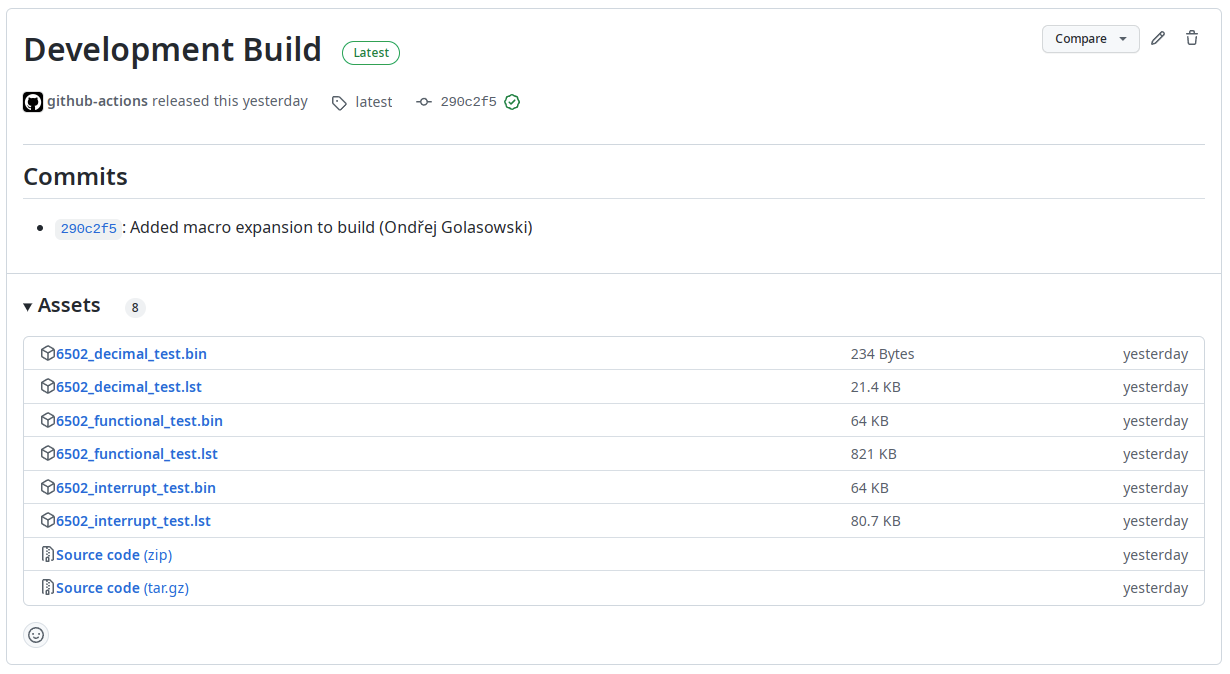
\includegraphics[width=0.8\textwidth]{images/vydani-testu-6502.png}
\end{figure}

\subsection{Integrace s Google Test}
Nakonfigurované a sestavené testy je nyní možné spouštět ručně. Pro automatické spouštění je nutné vytvořit testovací funkci pro platformu Google Test. Aby byly dodržovány zásady dobrého testování, je vhodné test vytvořit za použití existující komponenty, do které se nebudou přidávat žádné funkcionality pouze pro běh testu. Případné změny lze totiž provést přímo v~testu, a~to za použití dědičnosti. Ve výpisu~\ref{list:6502-test-uprava} je znázorněna upravená třída procesoru. Je použit název DUT (design under test), který se používá například při tvorbě testů ve VHDL. Důležitou úpravou je přidání rozhraní pro úpravu programového čítače, což je nutné pro spuštění testu a~kontroly stavu testu.

\begin{listing}
	\caption{Upravený procesor 6502 v Google Test}
	\label{list:6502-test-uprava}
	\begin{minted}{c++}
    class DUT : public MOS6502 {
	public:
	void step() {
		while(!instrFinished()) {
			CLK();
		}
		CLK();
	}
	uint16_t getPC() {
		return m_registers.pc;
	}
	void setPC(uint16_t val) {
		m_registers.pc = val;
	}
	void triggerNMI() {
		NMI();
	}
	void setIRQ(bool active) {
		IRQ(active);
	}
};
	\end{minted}
\end{listing}

Samotný test pak probíhá v~jednoduchém cyklu, kde podmínkou pro opuštění je opakovaná hodnota programového čítače. Ověření výsledku probíhá porovnáním poslední hodnoty programového čítače. Dle listingu vygenerovaného assemblerem lze zjistit, že úspěch je signalizován zacyklením na adrese \mintinline{text}|$06e5|, což ukazuje výňatek ve výpisu~\ref{fig:6502-test-uspech}. Celý testovací cyklus s~ověřením výsledku se nachází ve výpisu~\ref{list:6502-test-cyklus}.

\begin{listing}
	\caption{Řádek signalizující úspěch v listingu testu 6502}
	\label{fig:6502-test-uspech}
	\begin{minted}{ca65}
                                success         ; Navesti makra uspechu.
06e5 : 4ce506          >        jmp *           ; Test byl dokoncen uspesne.
	\end{minted}
\end{listing}

\begin{listing}
	\caption{Testovací cyklus procesoru 6502 v Google Test}
	\label{list:6502-test-cyklus}
	\begin{minted}{c++}
do {
	prevPC = cpu.getPC();
	cpu.step();
} while(prevPC != cpu.getPC());

EXPECT_EQ(prevPC, ADR_SUCCESS) 
	<< "The test failed on trap at address 0x"
	<< std::hex << prevPC;
	\end{minted}
\end{listing}


\subsection{Příklad testování}
Jedním z~problému, které se v~průběhu vývoje objevily, byl problém s~časováním přerušení. Byla proto vytvořena verze, která lépe odpovídá skutečnému chování. Kvůli tomu ale přestal fungovat test přerušení: \mintinline{text}|6502_interrupt_test.bin|. Tato část popisuje, jak se dá podobná chyba diagnostikovat a~opravit.

Test se zastavil na adrese \mintinline{text}|$6b2|. Dle listingu tato adresa odpovídá sekci, kde se testují oba přerušení, NMI a~IRQ. Část způsobující chybu je vyobrazena ve výpisu~\ref{list:6502-test-hledani-chyby}. Nejprve se nastaví vyvolání obou typů přerušení instrukcí \mintinline{text}|sta I_port|, přičemž IRQ bylo maskováno (pro stručnost není proces maskování uveden). Čeká se na provedení obslužné rutiny NMI a~otestuje se, zdali proběhlo. Poté se povolí přerušení IRQ instrukcí \mintinline{text}|cli|. Nyní by měla proběhnout rutina IRQ, k~tomu však nedojde a~test se zastaví.

\begin{listing}
	\caption{Příklad konfigurace testu pro procesor 6502}
	\label{list:6502-test-hledani-chyby}
	\begin{minted}{ca65}
; Testovani IRQ a NMI s maskovanim preruseni.
; ...
												; Testovani NMI
0699 : 8dfcbf          >        sta I_port      ; Vyvolani preruseni.

069c : e8                       inx
069d : e8                       inx
069e : e8                       inx
069f : ad0302                   lda I_src       ; Probehlo preruseni?
                                trap_ne
06a2 : d0fe            >        bne *           ; Pokud ne, skonci test.

06a4 : a200                     ldx #0

06a6 : a902                     lda #2          ; Testovani IRQ
06a8 : 8d0302                   sta I_src
06ab : 58                       cli             ; Povoleni IRQ.
06ac : e8                       inx
06ad : e8                       inx
06ae : e8                       inx
06af : ad0302                   lda I_src       ; Probehlo preruseni?
                                trap_ne
06b2 : d0fe            >        bne *           ; Pokud ne, skonci test.
	\end{minted}
\end{listing}

Již na základě této množiny informací lze chybu nalézt. Test nastaví zpětnovazební registr tak, aby byla vyvolána oba přerušení již při prvním testu, kdy se ověřuje NMI. V~dalším testu (ověření IRQ) již pouze povolí přerušení a~hodnotu ve zpětnovazebním registru nemění.

Skutečný procesor 6502 každé přerušení detekuje jiným způsobem. Přerušení IRQ detekuje úrovňový detektor. Při logické nule se zaznamená požadavek na přerušení a~po dokončení stávající instrukce se ověří, zdali přerušení není maskováno. Pokud je, provede se další instrukce normálním způsobem a~požadavek se zahodí. Tento požadavek je ale znovu zaznamenán, pokud je signál stále aktivní (tedy na logické nule). Emulovaný procesor vyvolal při zápisu do zpětnovazebního registru pouze jeden požadavek, choval se tedy jako hranový detektor, což je v~rozporu se skutečným procesorem, a~proto toto chování test vyhodnotil jako chybné. Hranový detektor je použit pouze u~NMI.

Stačí tedy funkci odpovídající pinu IRQ implementovat tak, aby se dal nastavovat jeho stav (aktivní a neaktivní), nikoliv pouze vyvolávat signál, jako je to u~NMI. Klíčovou část kódu ukazuje výpis~\ref{list:6502-preruseni-irq-oprava}.

\begin{listing}
	\caption{Oprava chybné implementace IRQ}
	\label{list:6502-preruseni-irq-oprava}
	\begin{minted}{c++}
void MOS6502::IRQ(bool active){
	m_irq = active;
}
	\end{minted}
\end{listing}


\begin{note}[Funkčnost původní implementace]
A proč tedy původní implementace fungovala? To bylo způsobeno jinou chybou, kdy se požadavek na přerušení ukládal, pokud bylo přerušení maskováno. To ale také neodpovídá skutečnému procesoru.
\end{note}

\subsection{Další testy}
TODO Popsat nestest a další.
